% Gemini theme
% https://github.com/anishathalye/gemini

\documentclass[final]{beamer}

% ====================
% Packages
% ====================

\usepackage[T1]{fontenc}
\usepackage{lmodern}
\usepackage[size=custom,width=120,height=72,scale=1.0]{beamerposter}
\usetheme{gemini}
\usecolortheme{gemini}
\usepackage{graphicx}
\usepackage{booktabs}
\usepackage{subfigure}
\usepackage{tikz}
\usepackage{amssymb}
\usepackage{amsmath}
\usepackage{pgfplots}

% ====================
% Lengths
% ====================

% If you have N columns, choose \sepwidth and \colwidth such that
% (N+1)*\sepwidth + N*\colwidth = \paperwidth
\newlength{\sepwidth}
\newlength{\colwidth}
\setlength{\sepwidth}{0.025\paperwidth}
\setlength{\colwidth}{0.3\paperwidth}

\newcommand{\separatorcolumn}{\begin{column}{\sepwidth}\end{column}}

% ====================
% Title
% ====================

\title{Panviral Pepseq: A Highly Multiplexed Serological Diagnostic}

\author{Zane Fink\inst{1} \and Jason Ladner\inst{1}}

\institute[shortinst]{\inst{1} The Pathogen and Microbiome Institute at Northern Arizona University}

% ====================
% Body
% ====================

\begin{document}

\begin{frame}[t]
\begin{columns}[t]
\separatorcolumn

\begin{column}{\colwidth}

  \begin{block}{Abstract}

Viruses represent a diverse and ubiquitous challenge to the immune system, and a record of these encounters is preserved within our antibody responses. 
Understanding the diverse antiviral immune response has important implications for both epidemiology and immunology, 
but our capacity for characterizing this response has been historically limited due to the low throughput nature of the available assays. 
To circumvent these limitations, we are developing a high-throughput approach for serological characterization that begins with a custom set of oligonucleotides (oligos),
which are ultimately linked to the peptides they encode, in order to allow for direct interaction with serum antibodies.
To aid in the design of these oligos, we have developed algorithms to optimize coverage of a given set of viral proteins using fewer oligos than current algorithms.
By treating the design of these libraries as an instance of the weighted set cover problem, 
we can iteratively select the oligos that best represent the potential epitopes within a given reference set. 
Using these algorithms, we were able to cover an equal amount of peptide diversity with $20\%$ fewer oligos. 
By increasing the efficiency of design algorithms, we are able to cover more viral diversity within a single assay, 
greatly increasing the sensitivity of a single assay.

\end{block}


\begin{alertblock}{Objectives}
  \begin{itemize}
  \item \textbf{Design} an oligo library for Ab-PepSeq that broadly
    covers viruses that infect humans/mammals.
  \item \textbf{Create} algorithms for the efficient coverage of
    \emph{linear epitopes} (i.e., in as few oligos as possible).
  \item \textbf{Implement} these algorithms in an open source
    easy-to-use software package that is freely available for public use.
  \end{itemize}
\end{alertblock}
  % \begin{block}{Hypothesis}
  %   \begin{itemize}
  %   \item By treating the design of an oligonucleotide library as an instance
  %         of the weighted set cover problem, we can cover a grater range of epitope diversity
  %         in a smaller set of designed oligos.
  %   \end{itemize}

  % \end{block}
  \begin{block}{Background: What is PepSeq?}
    \begin{figure}
      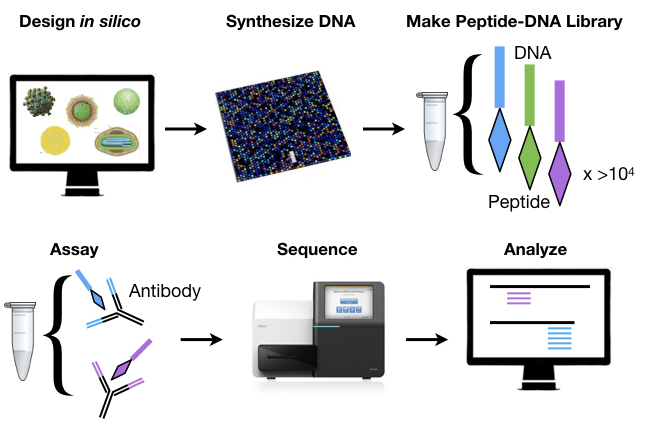
\includegraphics[width=0.6\colwidth]{figures/Overview.jpeg}
      \label{fig:library}
    \end{figure}
    \begin{itemize}
    \item Synthesize $100,000$s of DNA oligos that represent a diverse set of viral proteins.
    \item Serum antibodies used to enrich for recognized peptides
    \item Next-Generation Sequencing used for bulk characterization of enriched peptides.
    \item In this work we focus on the first step: \emph{Design in Silico}.

    \end{itemize}
  \end{block}

  \begin{block}{Who Cares? And Why You Should}
    \begin{itemize}
      \item This technology will have broad
            implications for the fields of infectious disease epidemiology, health equity and immunology, by providing a
            much broader view of the immunological response to infectious agents than was previously possible.
          \item  Due to the massive and rapidly evolving human virome,
            we need efficient algorithms to cover an incredibly diverse set of potential viral epitopes.

    \end{itemize}
  \end{block}
\end{column}

\separatorcolumn



\begin{column}{\colwidth}

\begin{block}{The Set Cover Problem}
  Consider a finite set $\mathcal{U}$ of elements, and a set $S$ of $k$ sets, where
  $\bigcup_{1 \leq i \leq k}S_i = \mathcal{U}$. We seek to cover the elements of $\mathcal{U}$ in as few
  sets of $S$ as possible.
  \vskip3ex
  \noindent
    \begin{minipage}{0.5\colwidth}
      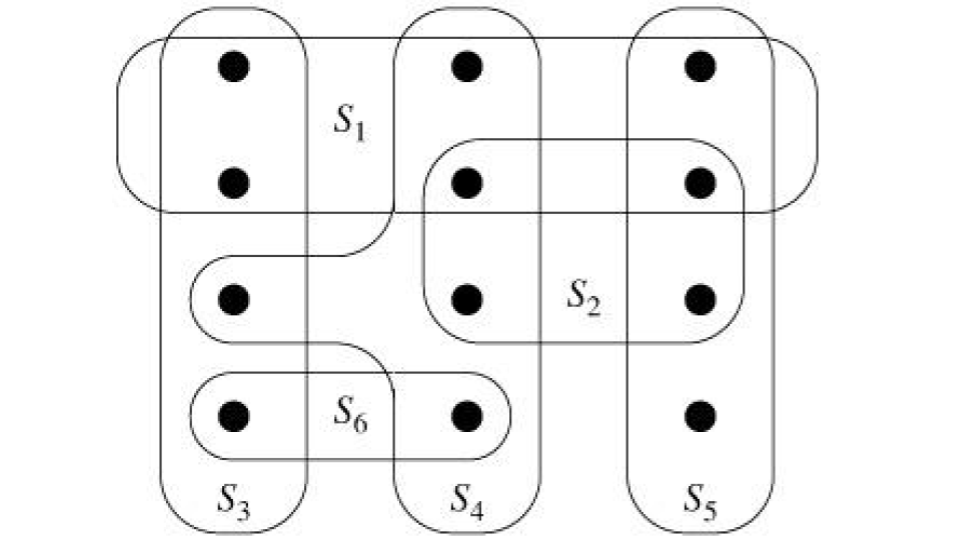
\includegraphics[height=8\baselineskip]{figures/set_cover.png}
    \end{minipage}%
    \begin{minipage}{0.5\colwidth}%
    \begin{itemize}%
      \item How we do cover all of the elements (black dots) of the above in as few sets as possible?
      \item \textbf{Greedy Algorithm}: Choose the largest set of uncovered items, the items in this set are now considered \emph{covered} and are no longer considered.
    \end{itemize}%
    \end{minipage}
\end{block}

\begin{block}{The Set Cover Problem As Applied to PepSeq}
    \begin{figure}
      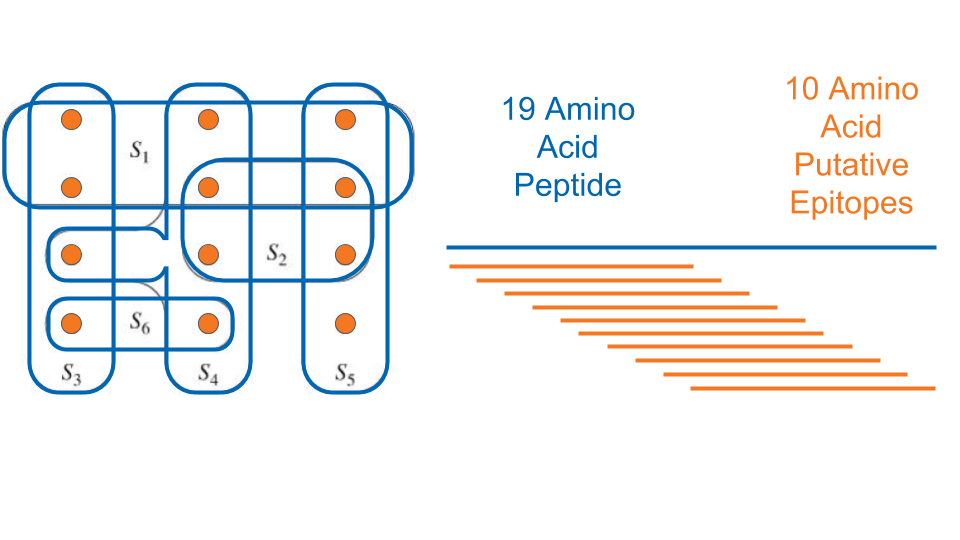
\includegraphics[width=0.7\colwidth]{figures/set_cover_oligo.png}
      \label{fig:library}
      % \caption{}
    \end{figure}
    \begin{itemize}
      \item Here we consider our Universe the set of $10$-mer linear epitopes in a set of viral proteins.
      \item We try to cover these epitopes using as few $19$-mer oligos as possible.
      \item Note that a single $19$-mer can cover up to $10$ unique $10$-mer linear epitopes.
      \item Polynomial time greedy algorithm results in long runtimes for larger datasets.
    \end{itemize}


\end{block}

\begin{block}{Another Approach: Naive Alignment-Based Sliding Window}
  We describe the sliding window approach as follows.
  Let $S$ be a set of aligned viral protein sequences, and let $k$ be the window size and $j$ the step size, where $1\leq j < k$.
  Then, the number $n_k$ of $k$-length subsequences of a sequence $s$ of length $p$ with step $j$ is $n_k = \lceil(p - k + 1 )/j\rceil$.
  We define $A = \{ s_{t\cdot k }s_{t\cdot k + j}, 0 \leq t < n_k$, for all $s \in S \}$, the set of subsequences of each sequence
  $s\in S$, where each subsequence is a $k$-mer with a step of $j$.

  \vskip1ex
  \noindent
  \begin{minipage}{0.7\colwidth}
    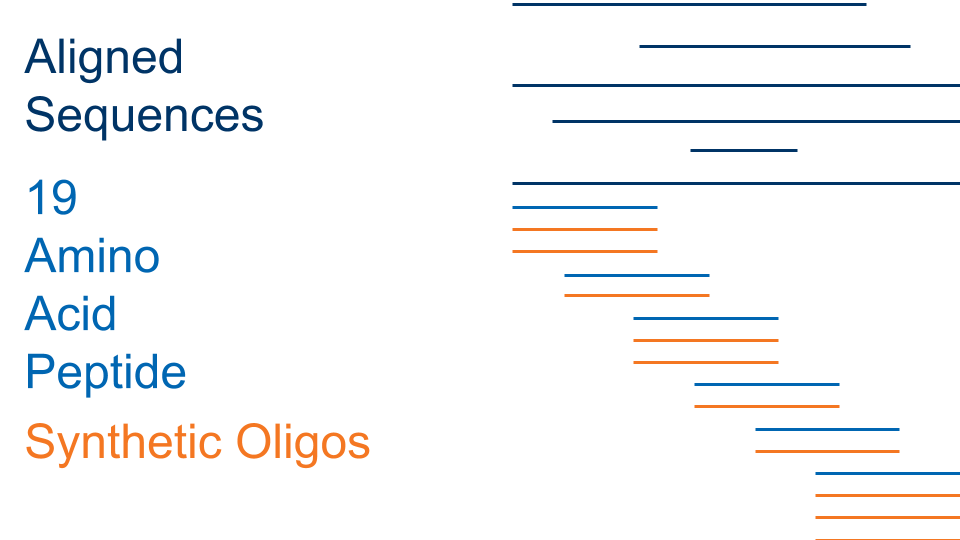
\includegraphics[height=12\baselineskip]{figures/sliding_window.png}
  \end{minipage}%
  \begin{minipage}{0.3\colwidth}
    \begin{itemize}
    \item In the naive approach, any oligos with gaps are immediately discarded. This results in a
      great reduction of epitope coverage.
    \item Once the alignment has been completed, runtime of this approach is very low. However, aligning
      large datasets can be very time consuming.
    \end{itemize}
  \end{minipage}

\end{block}

\end{column}

\separatorcolumn

\begin{column}{\colwidth}

  \begin{block}{Another Approach: Gap-Spanning Alignment-Based Sliding Window}
    \begin{figure}
      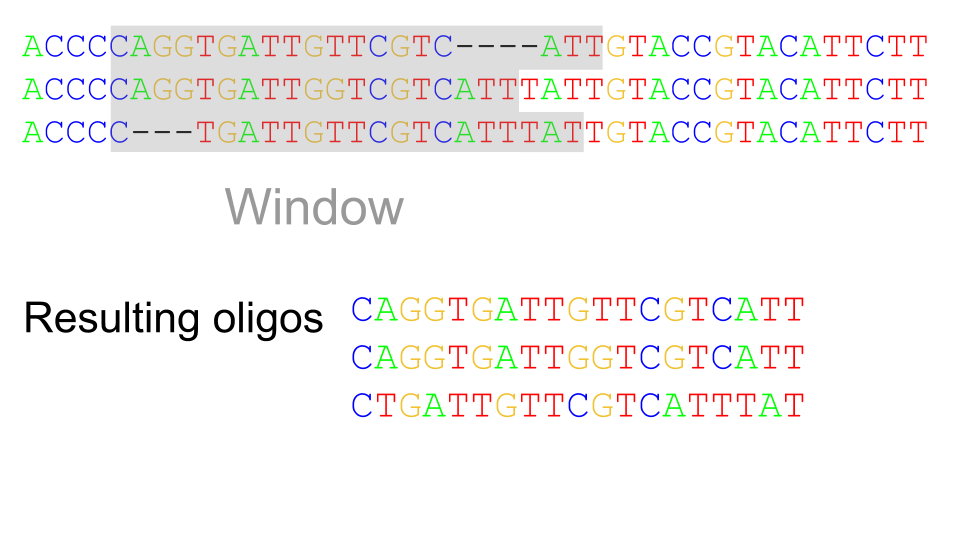
\includegraphics[width=0.8\colwidth]{figures/gap_spanning.png}
    \end{figure}

    \begin{itemize}
    \item Similar to \emph{Naive Alignment-Based Sliding Window}, but instead of discarding oligos with gaps,
          we span the gaps and keep the amino acids on either side of a gap.
      \item Results in far greater coverage than the \emph{Naive} approach but many more oligos than \emph{Set Cover}.
    \end{itemize}
  \end{block}

  \begin{block}{Results}
    \begin{minipage}[t]{0.5\colwidth}
        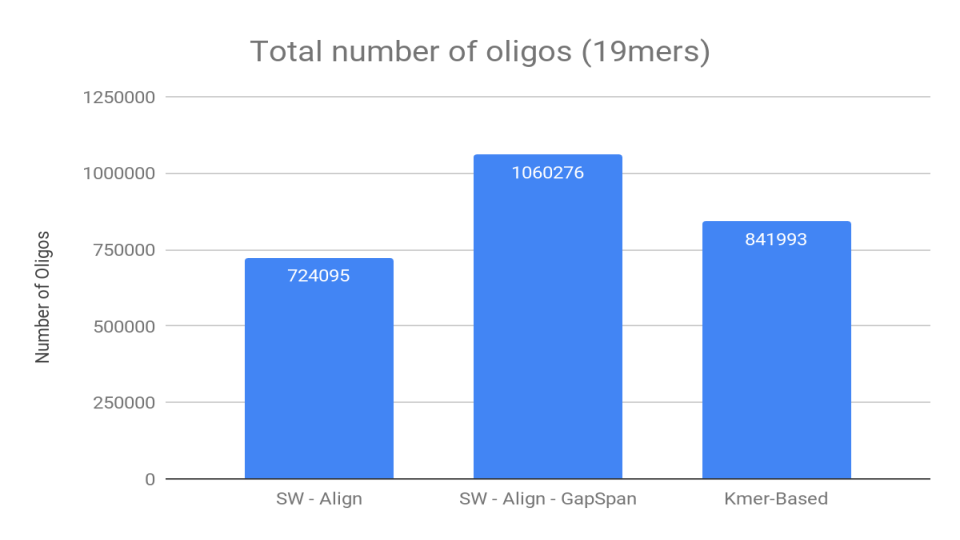
\includegraphics[width=0.5\colwidth,height=15\baselineskip]{figures/total_num_oligos.png}
    \end{minipage}%
    \begin{minipage}[t]{0.5\colwidth}
      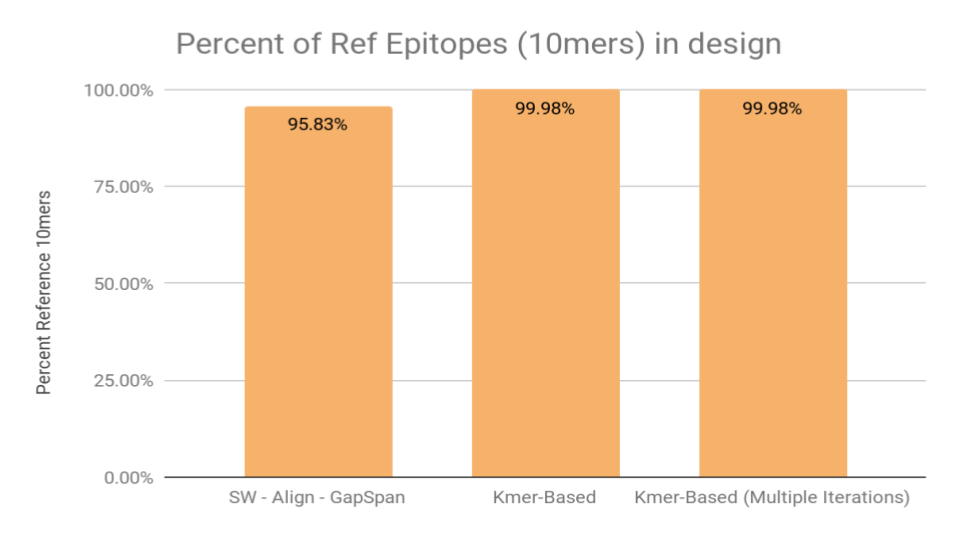
\includegraphics[width=0.5\colwidth,height=15\baselineskip]{figures/percent_ref_epis.png}
    \end{minipage}
  \end{block}

  \begin{block}{Conclusion}
    \begin{itemize}
    \item \emph{Set Cover} results in coverage of $4.15\%$ more $10$-mer epitopes than \emph{SW-Align w/ GapSpan}, and
           $21.22\%$ more $10$-mer epitopes than \emph{SW-Align}.
         \item \emph{Set Cover} covers $99.98\%$ of oligos in $841,993$ epitopes, while \emph{SW-Align w/ GapSpan} covers $95.83\%$ of epitopes in
           $20.6\%$ more oligos than \emph{Set Cover}.
    \end{itemize}

    \begin{block}{Next Steps}
      \begin{itemize}
      \item The designed peptide pool can now go through the process of being encoded as nucleotide sequences.
      \item These oligonucleotides will be synthesized and used to create a Peptide DNA Library, which
            will be used for probing for antiviral antibody immunological response in sera. 
      \end{itemize}
    \end{block}
  \end{block}
\end{column}

\separatorcolumn
\end{columns}
\end{frame}

\end{document}
